%\documentclass[tikz,border=2mm]{standalone}
\documentclass[tikz,border=2mm]{standalone}

\usepackage{amsmath}
\usepackage{amssymb}
\usepackage{subfigure}
\usetikzlibrary{shapes.geometric}
\usepackage[font=footnotesize]{caption}
\usepackage{pgfplots}
\usepackage{tikz}

\usetikzlibrary{shapes,backgrounds}

\newcommand{\tstar}[5]{% inner radius, outer radius, tips, rot angle, options
\pgfmathsetmacro{\starangle}{360/#3}
\draw[#5] (#4:#1)
\foreach \x in {1,...,#3}
{ -- (#4+\x*\starangle-\starangle/2:#2) -- (#4+\x*\starangle:#1)
}
-- cycle;
}

\newcommand{\ngram}[4]{% outer radius, tips, rot angle, options
\pgfmathsetmacro{\starangle}{360/#2}
\pgfmathsetmacro{\innerradius}{#1*sin(90-\starangle)/sin(90+\starangle/2)}
\tstar{\innerradius}{#1}{#2}{#3}{#4}
}

\usetikzlibrary{shapes.geometric}

\newcommand\score[2]{
\pgfmathsetmacro\pgfxa{#1+1}
\tikzstyle{scorestars}=[star, star points=5, star point ratio=2.25, draw,inner sep=1.3pt,anchor=outer point 3]
  \begin{tikzpicture}[baseline]
    \foreach \i in {1,...,#2} {
    \pgfmathparse{(\i<=#1?"yellow":"gray")}
    \edef\starcolor{\pgfmathresult}
    \draw (\i*1.75ex,0) node[name=star\i,scorestars,fill=\starcolor]  {};
   }
  \end{tikzpicture}
}

% Scriptsize axis style.
\pgfplotsset{every axis/.append style={tick label style={/pgf/number format/fixed},font=\scriptsize,ylabel near ticks,xlabel near ticks,grid=major}}

\begin{document}

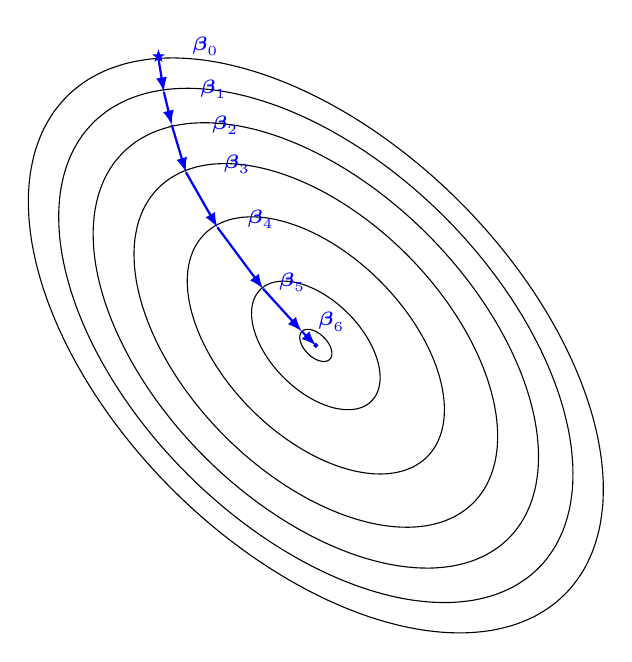
\begin{tikzpicture}[>= latex,samples=100,smooth]
	\begin{scope}
		\draw plot[domain=0:360] ({cos(\x)*sqrt(20/(sin(2*\x)+2))},{sin(\x)*sqrt(20/(sin(2*\x)+2))});
		\draw plot[domain=0:360] ({cos(\x)*sqrt(16/(sin(2*\x)+2))},{sin(\x)*sqrt(16/(sin(2*\x)+2))});
		\draw plot[domain=0:360] ({cos(\x)*sqrt(12/(sin(2*\x)+2))},{sin(\x)*sqrt(12/(sin(2*\x)+2))});
		\draw plot[domain=0:360] ({cos(\x)*sqrt(8/(sin(2*\x)+2))},{sin(\x)*sqrt(8/(sin(2*\x)+2))});
		\draw plot[domain=0:360] ({cos(\x)*sqrt(4/(sin(2*\x)+2))},{sin(\x)*sqrt(4/(sin(2*\x)+2))});
		\draw plot[domain=0:360] ({cos(\x)*sqrt(1/(sin(2*\x)+2))},{sin(\x)*sqrt(1/(sin(2*\x)+2))});
		\draw plot[domain=0:360] ({cos(\x)*sqrt(0.0625/(sin(2*\x)+2))},{sin(\x)*sqrt(0.0625/(sin(2*\x)+2))});
		
		
		\draw[->,blue, thick] (-2,3.65) to (-1.93,3.22);
		\draw[->,blue, thick] (-1.93,3.22) to (-1.83,2.8);
		\draw[->,blue, thick] (-1.83,2.8) to (-1.65,2.2);
		\draw[->,blue, thick] (-1.65,2.2) to (-1.25,1.5);
		\draw[->,blue, thick] (-1.25,1.5) to (-0.67,0.72);
		\draw[->,blue, thick] (-0.67,0.72) to (-0.18,0.18);
		%\draw[->,blue, thick] (-0.18,0.18); to (1.5,-0.5);
		\draw[->,blue, thick] (-0.18,0.18) to (0,-0);
		
		%\node[draw, fill, star, star points=5,minimum size=1mm] at (-2,3.6) {};
		%\ngram{4}{5}{45}{thick,fill=red}
		%\score{0}{1}
		\node[star,fill, blue,star points=5, star point ratio=2.6, draw,inner sep=0.5pt,anchor=outer point 3] at (-2.05,3.6) {};
		\node[circle,fill, blue, draw,inner sep=0.5pt] at (0,0) {};
		\node[blue] at (-1.4,3.8){\scriptsize $\boldsymbol{\beta}_0$};
		\node[blue] at (-1.3,3.25){\scriptsize $\boldsymbol{\beta}_1$};
		\node[blue] at (-1.15,2.8){\scriptsize $\boldsymbol{\beta}_2$};
		\node[blue] at (-1.0,2.3){\scriptsize $\boldsymbol{\beta}_3$};
		\node[blue] at (-0.7,1.6){\scriptsize $\boldsymbol{\beta}_4$};
		\node[blue] at (-0.3,0.8){\scriptsize $\boldsymbol{\beta}_5$};
		\node[blue] at (0.2,0.3){\scriptsize $\boldsymbol{\beta}_6$};
	\end{scope}
\end{tikzpicture}

\end{document}